\documentclass[tikz,border=3pt]{standalone}
\begin{document}
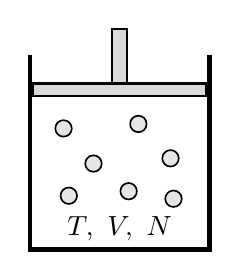
\begin{tikzpicture}[scale=0.95,line width=0.9pt]
  % 容器（底と左右の壁）
  \draw[line width=1.6pt] (-1.2,2.6) -- (-1.2,0) -- (1.2,0) -- (1.2,2.6);

  % ピストン
  \draw[fill=black!15] (-1.16,2.05) rectangle (1.16,2.22);
  \draw[fill=black!15] (-0.10,2.22) rectangle (0.10,2.95);

  % 気体分子
  \foreach \x/\y in {-0.75/1.62, 0.25/1.68, -0.35/1.15, 0.68/1.22, -0.68/0.72, 0.12/0.78, 0.72/0.68} {
    \draw[fill=black!10,line width=0.6pt] (\x,\y) circle (0.11);
  }

  % 状態量ラベル
  \node at (0,0.28) {$T,\ V,\ N$};
\end{tikzpicture}
\end{document}
